\documentclass[letter, 10pt]{article}
\usepackage[utf8]{inputenc}
\usepackage[spanish]{babel}
\usepackage{amsfonts}
\usepackage{amsmath}
\usepackage{graphicx}
\usepackage{grffile}
\usepackage{url}
\usepackage{caption}
\usepackage{subcaption}
\usepackage[top=3cm,bottom=3cm,left=3.5cm,right=3.5cm,footskip=1.5cm,headheight=1.5cm,headsep=.5cm,textheight=3cm]{geometry}
\usepackage[
    backend=biber,
    style=ieee,
    sorting=none
]{biblatex}
\usepackage{hyperref}
\hypersetup{
    colorlinks=true,
    linkcolor=cyan,
    filecolor=magenta,      
    urlcolor=cyan,
    citecolor=cyan,
    pdftitle={201954014-9-CristianSoriano-Ent1},
    pdfpagemode=FullScreen,
}

\addbibresource{Referencias.bib}

\begin{document}
\title{Inteligencia Artificial \\ \begin{Large}Estado del Arte: \textit{The Social Golfer Problem}\end{Large}}
\author{Cristian Soriano}
\date{\today}
\maketitle


%--------------------No borrar esta secci\'on--------------------------------%
\section*{Evaluaci\'on}

\begin{tabular}{ll}
Mejoras 2da Entrega (10 \%): &  \underline{\hspace{2cm}}\\
C\'odigo Fuente (10 \%): &  \underline{\hspace{2cm}}\\
Representaci\'on (5 \%):  & \underline{\hspace{2cm}} \\
Descripci\'on del algoritmo (15 \%):  & \underline{\hspace{2cm}} \\
Experimentos (10 \%):  & \underline{\hspace{2cm}} \\
Resultados (40 \%):  & \underline{\hspace{2cm}} \\
Conclusiones (10 \%): &  \underline{\hspace{2cm}}\\
 &  \\
\textbf{Nota Final (100)}:   & \underline{\hspace{2cm}}
\end{tabular}
%---------------------------------------------------------------------------%
\vspace{2cm}


\begin{abstract}
\textit{The Social Golfer Problem} es un problema famoso en el campo de la optimización combinatoria. Este problema es esencial para todo lo que es organización de torneos tipo Round-Robin ya que en su forma más general trata de organizar mini torneos por la máxima cantidad de semanas posibles tal que ningún jugador se tope con otro más de una vez. En este informe se van a explorar los distintos enfoques que se le han dado al problema, tanto en modelos como en las técnicas que se han usado para resolverlo. El objetivo final es formar un punto de vista en base a la información recolectada para luego enfocarse netamente en probar distintas técnicas para encontrar soluciones guiándonos por lo que se tiene actualmente.
\end{abstract}

\section{Introducci\'on}

En este informe se hará una revisión y análisis del estado del arte de \textit{Social Golfer Problem} (abreviado SGP a lo largo del trabajo), un problema de optimización combinatoria que ha generado bastante discusión en términos de rupturas de simetrías en problemas similares. La tarea principal es organizar una cierta cantidad $gp$ de golfistas en $g$ grupos de $p$ jugadores durante $w$ semanas; generalmente queremos extender el torneo lo más posible por lo que se busca maximizar $w$. Partiremos con la definición del problema (\ref{def}), donde se da un contexto profundo de cómo se debería abordar el problema dado su origen, problemas similares que son instancias de SGP y variantes/generalizaciones que se han postulado en diversas investigaciones. En el estado del arte (\ref{stateart}) veremos los distintos enfoques que se han dado tanto en modelos y métodos de resolución, haciendo comparaciones en rendimiento según lo que se tiene a la fecha. En este informe también se exploran algunos modelos propuestos que han mostrado resultados interesantes dada su complejidad, vistos en \ref{mod}, haciendo comparaciones según lo que se encontró en el estado del arte. En \ref{rep} empezamos a armar una metodología para plantear nuestro propio algoritmo para resolver el problema. Luego en \ref{algdesc} definimos los distintos tipos de construcciones que se quieren aplicar, en conjunto con un componente de búsqueda local con el algoritmo Hill Climbing. Para poner a prueba la metodología planteada en \ref{exps} definimos experimentos cruciales para medir el rendimiento de nuestro algoritmo y saber qué parámetros son ideales para este para luego en \ref{results} mostrar los resultados obtenidos de los experimentos. Finalmente haremos notar las conclusiones (\ref{conc}) relevantes que se pudieron sacar de este estudio, dando también posible trabajo a futuro por realizar.

\section{Definici\'on del Problema} \label{def}

En \cite{SolTriska1} se define al SGP como un problema de optimización combinatoria que surge de una pregunta publicada en \texttt{sci.op-research} en mayo de 1998: \textit{32 golfistas juegan golf una vez a la semana, siempre en grupos de a 4. ¿Por cuántas semanas pueden hacer esto tal que dos golfistas no jueguen en el mismo grupo más de una vez?}

En el mismo libro se plantea una generalización de SGP con el siguiente problema de decisión: ¿Es posible programar $g\times p$ golfistas en $g$ grupos de $p$ jugadores por $w$ semanas tal que dos golfistas no jueguen en el mismo grupo más de una vez?\\
Una instancia de SGP se denota mediante una tripleta $g-p-w$. La instancia original del problema se denotaría como $8-4-w$, donde $w$ sería la cantidad de semanas donde se cumplen las condiciones. En adición a todo esto, también se puede considerar a SGP como un problema de optimización discreta que maximiza el número de semanas $w^*$ para $g$ y $p$ dados, donde $w^*\leq \frac{g\cdot p - 1}{p - 1}$, es decir, la cantidad de semanas óptima no sobrepasa la cantidad de parejas únicas que pueden formarse en todos los grupos \cite{GolferRevisitedLiu}.  

El problema en sí es altamente combinatorio y simétrico por lo que no es sorprendente que haya llamado la atención por parte de la comunidad de programación con restricciones. Ha planteado problemas interesantes dentro del modelado y el quiebre de la simetría, volviéndose uno de los puntos de referencia estándar para evaluar esquemas que rompen la simetría de un problema \cite{dotu2005scheduling}.

Instancias conocidas de SGP son los \textit{Cuadrados de Euler} y el problema de \textit{Kirkman}. El primero, también conocido como el problema de los 36 oficiales, es la instancia $6-6-4$ de SGP, conocida por ser imposible \cite{SolTriska1}. El problema es el siguiente: \textit{Seis oficiales de 6 rangos distintos son elegidos de seis regimientos distintos. Se requiere arreglarlos en un cuadrado sólido tal que ningún oficial del mismo rango o del mismo regimiento se encuentre en la misma fila o columna}. Es un equivalente a arreglar 36 pares de enteros, cada uno menor o igual a seis, en un arreglo cuadrado tal que el primer (o segundo) número de los pares en cualquier fila o columna sean todos distintos, y que ninguno de 2 pares sean idénticos \cite{EulerOfficer}.

El segundo problema, también conocido como el problema de las quince alumnas, es la instancia $5-3-7$ de SGP, cuya descripción es la siguiente: \textit{Encontrar un calendario semanal para quince alumnas que salen a caminar a diario en cinco filas de tres alumnas cada una, de tal manera que dos chicas no deben caminar en la misma fila más de una vez por semana}. Una forma equivalente a la última parte es que \textit{cualquier alumna debe caminar exactamente una vez en la misma fila con cada una de las otras chicas}. Es conocido por ser uno de los problemas más importantes, celebrado y fascinante en el campo de las combinatorias y las matemáticas recreativas \cite{PAVONE2023113316}.

Otra instancia de SGP es \textit{The Social Doubles Tournament Problem} (SDTP), el problema consiste en crear un torneo tipo round robin (cada participante se encuentra con los demás) donde los equipos, compuestos por pares de jugadores, no están fijados a priori pero tienen que ser generados mientras se crean los rounds y donde cada jugador debe tener a todos los otros jugadores como compañero y como oponente. Además se pide que siempre que 4 jugadores se encuentren, hacer que se sigan encontrando durante tres partidos consecutivos en un mini torneo donde los jugadores cambian compañeros. En \cite{salassaa2017social} se encontró que, para $4n$ jugadores un torneo round robin prevé $4n-1$ rondas. Como cada cuádrupla determina 3 rounds para cada jugador, el número de rondas disjuntas totales es $\frac{4n-1}{3}$ y debe ser un número entero. Debido a esto, SDTP permite que existan soluciones factibles para $4n$ jugadores y se denota que SDTP$_{4n}$ es equivalente a la instancia $n-4-\frac{4n-1}{3}$ de SGP.   

SGP y problemas similares tienen varias aplicaciones prácticas, tales como desarrollos de frameworks para asignación de grupos, programación de grupos para salones de espera en zoom e incluso el estudio de la agrupación de torneos (como round-robin). Por ejemplo, en \cite{ACAD21SGP} se exploran soluciones a este problema con el uso de el sistema de numeros binarios en el torneo round-robin para asignar grupos de estudiantes en laboratorios y trabajos en grupo a lo largo de un semestre de un curso de química. Por otro lado, en \cite{MillerGroup21} se exploraron metodos para hacer las clases online durante la pandemia más didacticas, empleando uso de los salones de espera que ofrecía Zoom y Microsoft Teams para desarrollar actividades en grupo, donde se desea mezclar los grupos de tal manera que dos estudiantes no tuvieran el mismo grupo en más de una ronda, donde se uso una variación de SGP llamada \textit{Social Golfer Problem with Adjacent Group Sizes} (SGA), donde se busca asignar $v$ participantes a grupos con tamaños de $K$ (donde $K$ es un conjunto de enteros positivos de tamaño a lo más 2, si $|K|=2$ entonces $K=\{k,k+1\}$ para algún $k$) en $r$ rondas de tal manera que cada participante aparece en todas las rondas, todos los pares de participantes aparecen a lo más en un grupo y todas las rondas tienen el mismo conjunto de tamaños de grupos; es decir, se quiere encontrar un conjunto de rondas donde los tamaños de todos los grupos no necesariamente es el mismo. En otros casos se usan aplicaciones de otras variaciones de SGP, como en \cite{Lambers21Tournament}, donde se usa \textit{Traveling Social Golfer Problem} (TSGP), una generalización de SGP, para asignar grupos en la Volleyball Nations League, donde las dieciséis mejores naciones por genero compiten por un trofeo en un torneo que dura 6 semanas. En TSGP, definido en el mismo artículo, todos los grupos deben jugar en diferentes lugares, donde el objetivo es crear un calendario que minimiza la desigualdad (o injusticia) generada por los distintos tiempos de transporte entre las locaciones para cada golfista.

Ahora que tenemos un entendimiento base de SGP, podemos pasar a analizar distintas formulaciones del problema y cuales han sido las tendencias para encontrar soluciones a distintas instancias de éste.

\section{Estado del Arte} \label{stateart}

A lo largo de esta investigación nos hemos fijado que se han tomado muchos puntos de vista distintos para modelar y resolver el problema, desde propuestas de heurísticas greedy para obtener mejores resultados, hasta la ruptura de simetrías con el uso de teoría de conjuntos y con la suma de otras restricciones, mejorando el rendimiento a la hora de buscar soluciones.

En \cite{triska2012effective} se propone una mejora a lo que se propone en \cite{dotu2005scheduling}. Se introduce el concepto de grado de libertad de los jugadores, que, informalmente, denota con cuántos jugadores aún se puede emparejar al jugador. Esta métrica permite la mejora de dos métodos: bactracking completo y búsqueda local. Para el primer método, se plantea una heurística greedy que puede ser usada para guiar la búsqueda mediante backtracking para SGP. Si se asume que los jugadores por equipo $p$ es par, la tarea de asignar jugadores en grupos en cada semana es equivalente a organizar pares de jugadores dentro de grupos. De este modo, se visitan las semanas una tras otra y en cada semana se recorren los grupos en su orden natural. Por cada par de posiciones adyacentes en un grupo, se necesita seleccionar un par de jugadores que aún quedan por agrupar en la semana actual. Aquí se ocupa el grado de libertad para guiar la selección del par que tiene la mínima libertad con respecto a la configuración parcial actual. La intención detrás de esto es que si un par de jugadores esta cercano a quedarse sin potenciales parejas, entonces deben estar en el mismo grupo mientras sea posible. Si un grupo no puede ser completado, o se genera un conflicto, ocurre backtracking: se deshace la elección más reciente de jugadores y se selecciona un par con el mayor grado de libertad. Si $p$ es impar, se emparejan todos los jugadores posibles y después se rellena la posición que falta con cualquier jugador que sea compatible con el resto de jugadores que estén en el grupo. Otra opción sería usar tripletas y conjuntos de jugadores más grandes. La implementación de backtracking es tal que un patrón puede denotar de qué manera se considera a cada grupo por individual. Por ejemplo el patrón $3-2-2-1$ puede ser aplicado a instancias $g-8-w$ y significa que por cada grupo, se procede de la siguiente manera: primero se programa una tripleta de jugadores; en los lugares que quedan, se colocan dos pares inmediatamente después (cada uno elegido según la libertad mínima) y cualquier jugador que aún pueda jugar con todos en el grupo se pone en la posición final. En la figura \ref{fig:tabla1greedybt} se muestra la tabla con los resultados para las distintas instancias y patrones obtenidos con este método, por ejemplo, se resuelve el problema de Kirkman de manera óptima. También se resuelve el SGP original por 9 semanas con un patrón $2-2$ (dos pares) y 4 (considerando cuartetos).

\begin{figure}[h]
    \centering
    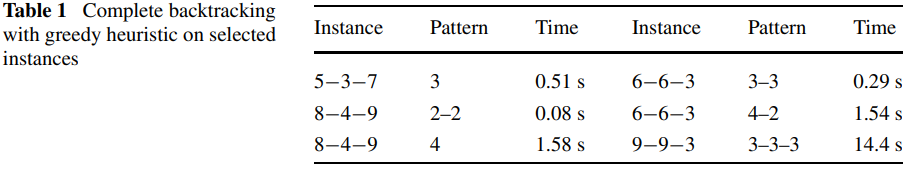
\includegraphics[width=\textwidth]{figures/table1_greedybt.png}
    \caption{Tabla con los resultados de la heurística con backtracking}
    \label{fig:tabla1greedybt}
\end{figure}

En el paper se usa la misma heurística greedy para generar configuraciones iniciales buenas para un enfoque de búsqueda local. Primero se usa una forma dual de la heurística definida, es decir, no garantiza encontrar la solución óptima pero si una cercana a ser óptima, en adición con un componente aleatorio que permite agregar pequeñas perturbaciones a las configuraciones iniciales. La heurística visita las semanas una tras otra. Una única semana se produce de la siguiente manera: Los grupos de esta semana se recorren uno tras otro. Al igual que antes, por cada par de posiciones adyacentes en un grupo, la heurística debe seleccionar un par de jugadores que aún deban ser asignados en la semana actual. Selecciona el par que tiene la libertad máxima con respecto a la configuración parcial actual. Hay un parámetro $\gamma$, con $0 \leq \gamma \leq 1$, que es usado para randomizar la heurística: En el caso que hayan empates, se realiza una elección aleatoria entre los pares de jugadores que tienen el máximo grado de libertad con probabilidad $\gamma$. Con probabilidad $1-\gamma$, los pares se consideran como ordenados, con el jugador con numeración más baja siendo primero, y se selecciona el par que es lexicográficamente más pequeño (el que tenga la letra que venga primero en el alfabeto). Después que un par de jugadores es seleccionado y asignado a un grupo, se substrae un número grande en forma de penalidad de la libertad de ese grupo en semanas siguientes, con esto se desalienta a que ese par sea seleccionado nuevamente en un grupo diferente. En otros casos, la heurística no presta atención a potenciales conflictos en un grupo, y nunca deshace una elección de pares. En el caso en que $p$ es impar, la heurística aún puede trabajar con pares de jugadores a excepción del último jugador en cada grupo. Con probabilidad $\gamma$, ese jugador es seleccionado de manera aleatoria de todos los jugadores que aún deben ser asignados en esa semana. Con probabilidad $1-\gamma$, el jugador cuya numeración es la más pequeña es seleccionado. Al igual que antes, la heurística es generalizada desde pares a conjuntos más grandes de jugadores, y nuevamente hay un intercambio entre maximizar la libertad de los grupos y la eficiencia. La intuición detrás de maximizar la libertad entre jugadores de un grupo es para hacer espacio a buenos movimientos locales, que serán discutidos en lo que sigue. Se apuntó a mantener el componente de búsqueda local lo más simple posible. Se usó el enfoque de un algoritmo memético, definido en \cite{cotta2006ma}, el cuál siguiendo la filosofía de la programación evolutiva, ocupa únicamente mutación como forma de diversificar la búsqueda, lo que alivia la necesidad de realizar rupturas de simetría; esto en conjunto con una base de búsqueda tabú. Se elimino la componente de reinicio debido a que se encontró innecesaria en experimentos: Incluso después de omitir la componente de reinicio, la búsqueda local implementada excedió los enfoques de búsqueda local reportados en la literatura. Sea que $C$ denota una configuración. La tripleta $(i,j,k)$ es una posición conflicto sí y solo sí dondequiera que un jugador esta en el mismo grupo con otro jugador más de una vez. Sea que $f(C)$ denote el número de posiciones conflicto en $C$. El rango de $f(C)$ es $[0,gpw]$. Un \textit{swap} que afecte a la posición $(i,j,k)$ significa el intercambio de los valores de $G_{ijk}$ con cualquier otro valor de alguna variable $G_{ij'k'}$, con $j'\neq j$ y $k'\neq k$, donde $G_{ijk}$ denota qué jugador juega en la semana $i$, grupo $j$ y posición $k$, con $0 \leq G_{ijk} \leq n=gp$. El movimiento es bueno ya que no rompe restricciones importantes del modelo usado. Una iteración de esta búsqueda local procede de la siguiente manera: Primero se determina $f=f(C)$. Si $f=0$, se encontró una solución y estamos listos. En caso contrario, de todos los swaps que afectan a las posiciones conflictivas, hacer el swap que lleve a una configuración $C'$ con $f(C')$ mínimos entre todas las configuraciones consideradas (rompiendo empates lexicográficamente). En adición, se asocia una lista tabú con cada semana que guarda todos los pares de jugadores que fueron intercambiados en las ultimas 10 iteraciones en esa semana. Swaps que afectan a un par de jugadores en la lista tabú de la semana correspondiente son considerados solamente si resultan en una mejora sobre la mejor solución encontrada hasta el momento. Si no hubo una mejora en las últimas 4 iteraciones, se hacen 2 swaps aleatorios. Se determinaron todos estos parámetros en pruebas sobre todas las instancias que se definieron en el artículo, y de todas esas, la configuración dada funcionaba mejor cuando se promedió sobre los tiempo de ejecución de todas las instancias probadas. En la figura \ref{fig:tabla2ts} se pueden ver los resultados obtenidos.

\begin{figure}[h]
    \centering
    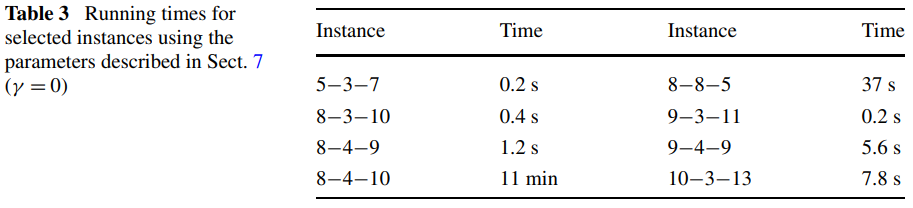
\includegraphics[width=\textwidth]{figures/table2_greedyts.png}
    \caption{Tabla con los resultados obtenidos usando búsqueda local}
    \label{fig:tabla2ts}
\end{figure}

La heurística usada es aleatoria y generalizada, y mostró que mejora resultados obtenidos mediante búsqueda local. Además de ser una de las más simples, es una de las más competitivas con otras meta heurísticas y técnicas basadas en restricciones en otras instancias.

En \cite{triska2008solving} se utiliza un \textit{greedy randomized adaptive search procedure} (GRASP) para resolver SGP. Dentro de una estructura básica de un GRASP para un problema de minimización, se adhiere al esquema con lo siguiente: La condición de termino es el descubrimiento de un horario sin conflictos (o un time out, cualquiera que ocurra primero); basándose en el mismo concepto de grado de libertad mencionado anteriormente (\cite{triska2012effective}), se generan las configuraciones iniciales con la misma heurística greedy aleatoria; Se usa la misma componente de búsqueda local que en el caso anterior, es decir, búsqueda tabú. Hay que notar que este estudio fue publicado antes que \cite{triska2012effective}, pero las especificaciones entre ambos son las mismas y cambian solamente en la parte de los resultados obtenidos. En este caso, la ejecución de una única instancia procede de la siguiente manera: La heurística greedy es usada para generar cinco condiciones iniciales variando $\gamma$, incluyendo 0, 0.1, 0.2 y dos valores sacados en momentos aleatorios entre 0.3 y 1. Luego, la componente de búsqueda local se ejecuta con cada una de las configuraciones obtenidas por a lo más un minuto. Si no se encuentra una solución, se reinicia la búsqueda con la configuración inicial que tenía el mínimo número de conflictos mientras era ejecutado, y luego es ejecutado hasta su finalización. Los resultados se muestran en la figura \ref{fig:grasptriska}. 

\begin{figure}[h]
    \centering
    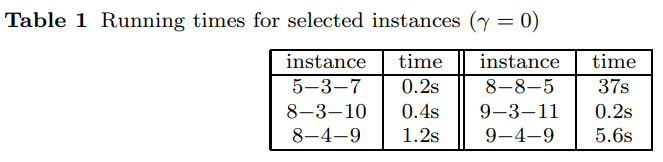
\includegraphics[width=0.8\textwidth]{figures/table4_grasp.png}
    \caption{Rendimiento de GRASP para instancias seleccionadas}
    \label{fig:grasptriska}
\end{figure}

Comparando con la figura \ref{fig:tabla2ts} los resultados obtenidos son bastante similares.

En \cite{barnier2005solving} se propone un modelo basado en programación entera y se rompen las simetrías durante la búsqueda para resolver el problema de Kirkman. Según este paper, las simetrías de SGP se pueden enumerar de la siguiente manera: 1) los jugadores pueden ser intercambiados dentro de los grupos; 2) los grupos pueden ser intercambiados dentro de las semanas; 3) Las semanas pueden ser ordenadas de manera arbitraria; 4) los jugadores pueden ser renombrados en $(gp)!$ permutaciones. Las restricciones que rompen simetrías fallan en remover estáticamente todas las simetrías entre los jugadores en SGP. En \cite{barnier2005solving} se especializa una técnica llamada \textit{Symmetry Breaking via Dominance Detection} (SBDD), la cual en su forma base consta en detectar puntos de elección simétricos dentro del procedimiento de búsqueda. Cada vez que el algoritmo de búsqueda genera un nuevo punto de decisión, se chequea si es equivalente a o dominado por un nodo que fue expandido antes. En ese caso, el punto de la decisión actual puede ser podado; caso contrario, se procede de forma normal \cite{fahle2001sym}. Este algoritmo requiere calcular una coincidencia en un grafo bipartito, para lo cuál el mejor algoritmo conocido corre en $\mathcal{O}(n^{\frac{5}{2}})$ \cite{hopkroft1973n5}. Sin embargo es significativamente más fácil chequear que existe una función que mapea una solución vieja (una hoja del árbol de búsqueda) a una nueva. En \cite{fahle2001sym} se remarca que las posibles simetrías pueden ser enumeradas buscando un match desde la primera semana de la primera solución (o solución parcial) hacia cualquier semana de la segunda solución. La idea clave para realizar el chequeo de la simetría de forma eficiente es hacerlo de manera floja: en lugar de elegir un matching completo y chequear las otras semanas después, vale la pena chequearlas mientras que el matching es construido. El chequeo para mapear pares puede ser rendido con un costo bajo con una fase de cálculos previos: 1) Derivar el conjunto de pares de cada semana $i$ de la primera solución $P$, ordenado de acuerdo al mayor elemento del par, denotado $C_i(P)$. Este cálculo puede llevarse a cabo solamente una vez que la solución es encontrada y guardada; 2) Construir una tabla de los números de la semana indexados por pares de la segunda solución $P'$. Un procedimiento eficiente de chequeos de simetría aplicado en las hojas permite calcular todas las soluciones únicas pero no mejora la búsqueda en sí: ningún subárbol es eliminado. Sin embargo, usando isomorfismos de grafos, se podría usar chequeos de simetría para podar subárboles grandes. En la figura \ref{fig:mckaypruned} se ilustra esta idea. Sea $P$ una solución inicial (el árbol se explora con depth first search, de izquierda a derecha) y $P'$ una segunda solución demostrada ser isomorfa a $P$ ($P' = \gamma(P)$ con $\gamma$ una biyección entre los vértices de $P'$ a $P$). Se denota $n=P\setminus P'$ como el nodo más profundo en el árbol de búsqueda que es común a los caminos desde la raíz a $P$ y $P'$, y a $s$ (respectivamente $s'$) su sucesor inmediato (se asume que el árbol de búsqueda es binario) que lleva a $P$. Se puede demostrar que el nodo $s'$ es la imagen de $s$ mediante el isomorfismo $\gamma$. En este caso, lo que falte por explorar del subárbol de $s'$ es la imagen de un subárbol ya explorado que empieza por $s$. Entonces puede ser podado porque solamente llevaría a soluciones que son imágenes por $\gamma$ de soluciones que ya se encontraron. A este idea se le conoce como poda profunda.

\begin{figure}[h]
    \centering
    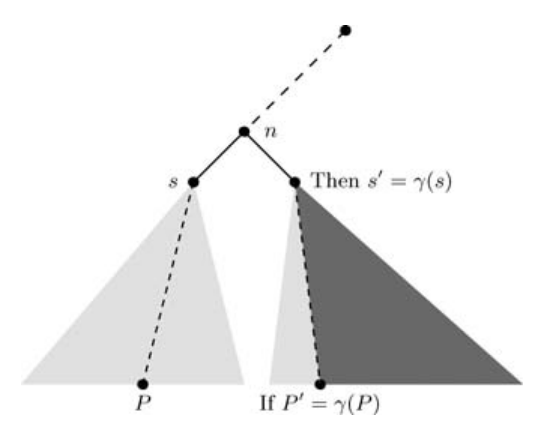
\includegraphics[width=0.4\textwidth]{figures/prunedMcKay.png}
    \caption{Árbol de búsqueda mencionado; El subárbol más oscuro puede ser podado}
    \label{fig:mckaypruned}
\end{figure}

En \cite{barnier2005solving} se propone una integración de poda profunda donde no solo se calculan los isomorfismos de las soluciones sino que también en estados del árbol de búsqueda que pueden ser descritos con los dominios actuales de las variables. A esta variación se le denomina SBDD+. El mismo algoritmo para chequear simetrías puede ser modificado fácilmente para ser aplicado a situaciones incompletas, intentando mapear la primera semana de la solución inicial solo en la primera semana de la segunda. La fase de chequeo se mantiene igual, una simetría se encuentra si todos los pares en $P$ tienen una imagen en $P'$. El chequeo de la dominancia sigue siendo costoso y no debe ser realizado tan seguido. La frecuencia de chequeo debe estar relacionada a la estructura del problema. Una buena premisa para SGP es guardar nodos en cada profundidad del árbol de búsqueda, chequear dominancia para nodos solamente contra nodos de profundidad más pequeña y chequear dominancia solo para nodos en profundidades que son múltiplos de $p$. La profundidad del árbol de búsqueda es el número de golfistas $gp$; en cada nivel, pueden haber $g^w$ nodos por guardar. El tamaño de todos los nodos que se guardan está delimitado por $gpg^w$. Este límite es malo debido a las numerosas simetrías que son removidas por las restricciones. Para el problema de Kirkman solo se guardan 15 nodos al mismo tiempo. La figura \ref{fig:sbdd+} ilustra el método en cuestión.

\begin{figure}
    \centering
    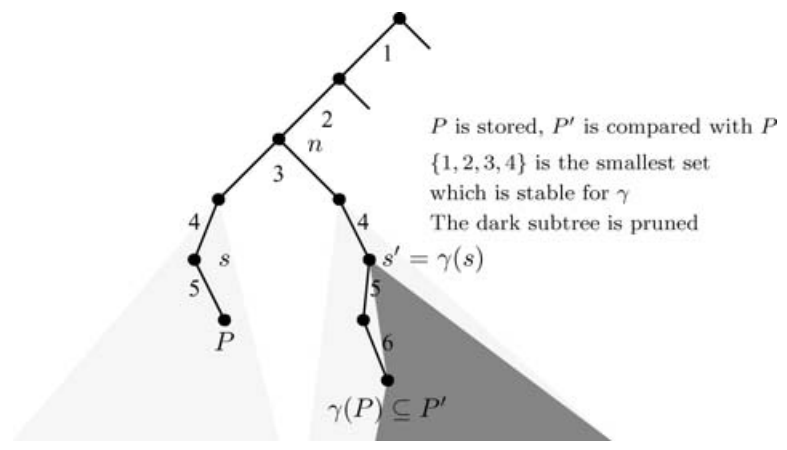
\includegraphics[width=0.5\textwidth]{figures/sbdd+.png}
    \caption{Poda profunda con SBDD}
    \label{fig:sbdd+}
\end{figure}

En la figura \ref{fig:table3kirkman} se puede ver el número de puntos de decisión creados, la cantidad de \textit{backtracks}, el total de soluciones encontradas, el número de chequeos de dominancia y el tiempo de CPU para diferentes combinaciones de métodos presentados para calcular las 7 soluciones del problema de Kirkman (que se hayan encontrado 11 soluciones significa que se detecto el isomorfismo solamente en la hoja del árbol de búsqueda). Los métodos +(4) y +(5) se refieren a la adición de restricciones redundantes al modelo con el objetivo de reducir la cantidad de backtacks. 

\begin{figure}[h]
    \centering
    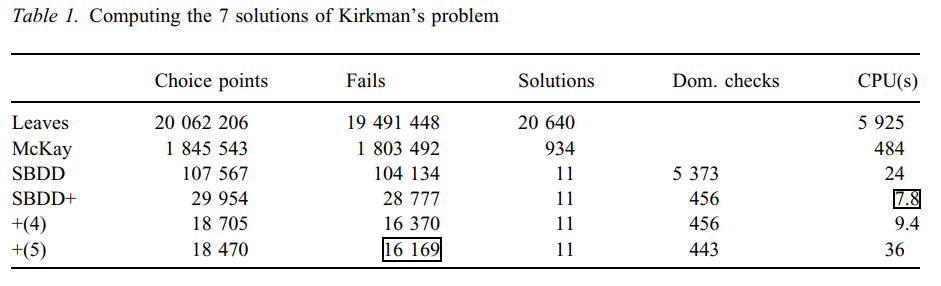
\includegraphics[width=\textwidth]{figures/table3_sbdd.png}
    \caption{Tabla comparativa entre los métodos usados}
    \label{fig:table3kirkman}
\end{figure}

En una investigación más reciente (\cite{lester21pb}), se formula un modelo parcialmente booleano (PB) de SGP para encontrar una configuración para un torneo de Mahjong. El uso de un modelo PB sobre la formulación SAT es debido a que el modelo SAT de este problema (que veremos en la sección de modelos matemáticos) para una cantidad grande de jugadores es muy lenta para generar las restricciones. Se asume que, mientras que un PB pueda no encontrar una solución óptima global, si dejó de encontrar mejoras, al menos habrá encontrado una solución óptima local. Además se asegura que a la fecha del paper, el método automatizado desarrollado en \cite{triska2012effective} es el mejor, aunque el método SAT/PB es competitivo. Una de las restricciones de este caso particular es el balance del viento (durante cada ronda a cada jugador se le asigna un punto cardinal distinto, conocido como viento): Con el fin de compartir una penalidad potencial de no tener un segundo turno siendo dealer a través de todos los jugadores, cada jugador debe ser alocado a cada posición inicial del viento aproximadamente el mismo número de veces. Para calendarios de torneos que corresponden a instancias duras de SGP, se puede importar una solución de la instancia y simplemente sintonizar el balance del viento. Una vez definido un enncoding para restricciones con los vientos (en la sección de modelos matemáticos se entrara en más detalle), se usa para generar calendarios para el torneo European Riichi Mahjong Championship (ERMC) del año 2016 y varios torneos más pequeños en el Reino Unido. La instancia de SGP que describe el torneo ERMC es la $32-4-10$ y se usa el encoding desarrollado, encendiendo (o habilitando) las restricciones de manera incremental para obtener los mejores resultados. Forzar a que ocurra la socialización (cada jugador debe jugar contra todos los demás) de por si solo tomó 18s. Se habilito el movimiento de las mesas y el balance del viento para darle a cada jugador 2 turnos en cada asiento más 1 turno como Este o Sur y 1 turno como Oeste o Norte, lo que tomo 2m con 10s en resolver. Manteniendo una restricción dura y agregando otra blanda, con un tiempo límite de 1 hora, se generó un calendario que no respeta 122 de $\binom{128}{2}=8128$ restricciones blandas. En general la instancia ocupó 1.3M de variables y 3.9M de restricciones y en la figura \ref{fig:enter-table6} se muestran puntos de referencia para instancias similares. A modo de comparación, resolver la instancia con búsqueda local balanceando los vientos usando la formulación propuesta produjo una solución en menos de 1 s. Para los torneos más pequeños, el grafo del torneo era más pequeño por lo que no se forzó con restricciones. Torneos de 1 día solían tener 5 sesiones y tenían de 24 a 52 jugadores ($6-4-5$ a $13-4-5$). Torneos de 2 días solían tener 8 sesiones y de 32 a 68 jugadores ($8-4-8$ a $17-4-8$). Se comparo la formulación monolítica con estos intervalos, con un tiempo máximo de 10 minutos para el solver y haciendo que el balance del viento sea una restricción suave. Para instancias en el intervalo de 1 día se tomo menos de 0.5s para resolver restricciones para un calendario con máxima socialización, movimiento de mesas y balance del viento, a excepción de $6-4-5$, la cuál tomó 3.6s. Para intervalos de 2 días (ver figura \ref{fig:table5}), la instancia $8-4-8$ es significativa ya que es la formulación original de SGP y queda fuera del alcance para la formulación SAT y PB, por lo que se importó una solución para balancear. Para $9-4-8$ y $10-4-8$, \textit{clasp} resolvió las restricciones solo con el balance del viento deshabilitado. Para el resto, \textit{clasp} encontró soluciones sin respetar de 2 a 21 restricciones con el viento. En todos los casos se pudo sintonizar perfectamente el balance del viento, satisfaciendo todas las restricciones, usualmente en menos de 2s. 

\begin{figure}[h]
    \centering
    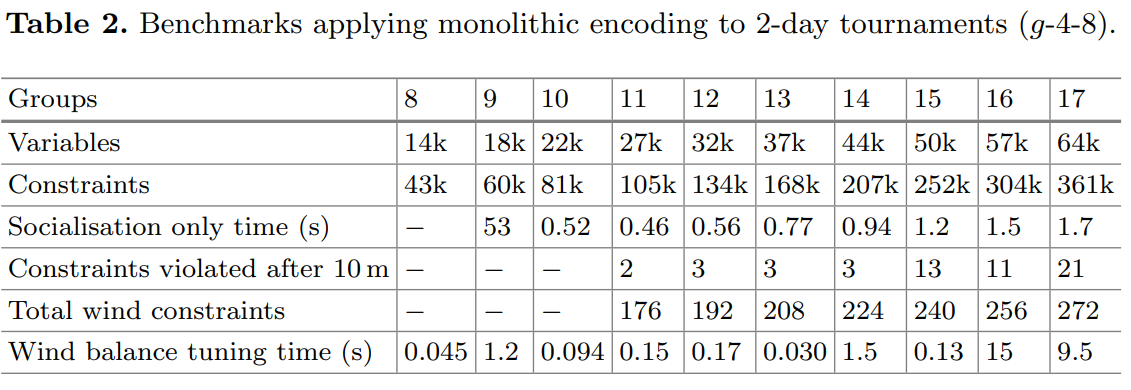
\includegraphics[width=0.8\textwidth]{figures/table5_monolithic.png}
    \caption{Puntos de referencia aplicando el encoding para torneos de 2 días}
    \label{fig:table5}
\end{figure}

\begin{figure}[h]
    \centering
    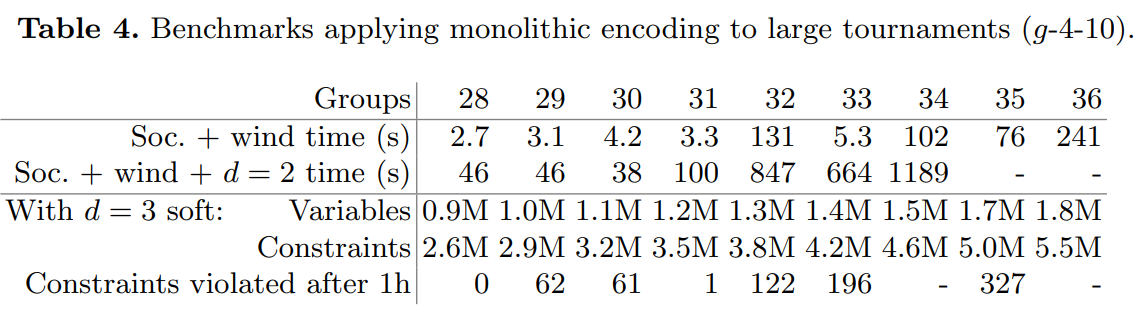
\includegraphics[width=0.8\textwidth]{figures/table6_monolithic.png}
    \caption{Instancias similares al torneo ERMC 2016}
    \label{fig:enter-table6}
\end{figure}

\section{Modelos Matemáticos} \label{mod}
Como lo prometido es deuda, empezaremos con los modelos que se consideran más simples y vamos a ir escalando un poco la dificultad a medida que revisemos más modelos. Partimos revisando una formulación SAT de SGP, la cual es una versión mejorada de un modelo previo. En \cite{triska2012improved}, consideramos $x=gp$ golfistas. La formulación original introduce variables $G_{ijkl}$ ($1\leq i \leq x, 1\leq j \leq p, 1\leq k \leq g$ y $1\leq l \leq w$) que denotan si es que el jugador $i$ juega en la posición $j$ en el grupo $k$ y semana $l$. Notar que en total tenemos $xpgw$ variables cada una con 2 valores posibles, por lo que la cardinalidad del espacio de búsqueda (hasta ahora) es de $2^{xpgw}$. Las restricciones se imponen en forma de clausulas asegurando que:
\begin{itemize}
    \item Cada jugador juega exactamente una vez a la semana:
    \begin{itemize}
        \item Cada jugador juega por lo menos y a lo más una vez por semana
    \end{itemize}
    \item Cada grupo consiste de exactamente p jugadores
    \item Dos jugadores no juegan en el mismo grupo más de una vez
\end{itemize}

A modo de nota, las clausulas establecen condiciones que deben cumplirse dentro de un conjunto de proposiciones (las restricciones de SGP, en este caso). Especifican cómo ciertas combinaciones de variables deben ser verdaderas (o falsas) para satisfacer estas proposiciones.
Las siguientes clausulas se aseguran de que cada jugador juega al menos una vez a la semana:

\begin{equation}
    \bigwedge_{i=1}^{x} \bigwedge_{l=1}^{w} \bigvee_{j=1}^{p} \bigvee_{k=1}^{g} G_{ijkl}
    \label{eq:1}
\end{equation}

Para asegurarnos que cada jugador juega a lo más una vez a la semana, primero nos debemos asegurar que cada jugador juegue a lo más una vez por grupo en cada semana:

\begin{equation}
    \bigwedge_{i=1}^{x} \bigwedge_{l=1}^{w} \bigwedge_{j=1}^{p} \bigwedge_{k=1}^{g} \bigwedge_{m=j+1}^{p} \neg G_{ijkl} \vee \neg G_{imkl}
    \label{eq:2}
\end{equation}

Un segundo conjunto de clausulas se supone que debe garantizar que ningún jugador juegue en más de un grupo en cualquier semana:

\begin{equation}
    \bigwedge_{i=1}^{x} \bigwedge_{l=1}^{w} \bigwedge_{j=1}^{p} \bigwedge_{k=1}^{g} \bigwedge_{m=k+1}^{g} \bigwedge_{n=j+1}^p \neg G_{ijkl} \vee \neg G_{inml}
    \label{eq:3}
\end{equation}

Sin embargo, el conjunto de clausulas en \ref{eq:3} es incompleto; en la versión modificada se cambia por:

\begin{equation}
    \bigwedge_{i=1}^{x} \bigwedge_{l=1}^{w} \bigwedge_{j=1}^{p} \bigwedge_{k=1}^{g} \bigwedge_{m=k+1}^{g} \bigwedge_{n=1}^p \neg G_{ijkl} \vee \neg G_{inml}
    \label{eq:4}
\end{equation}

El cambio realizado es que $n$ debe ir de 1 hasta $p$ en vez de $k+1$ a $p$, esto debido a que un jugador que juega en la semana $l$ en la posición $j$ en el grupo $k$ no debe jugar en cualquier otra posición para futuros grupos de esa semana, no posiciones mayores a $j$. Tomando la modificación presentada en consideración, el conjunto de clausulas \ref{eq:1} $\cup$ \ref{eq:2} $\cup$ \ref{eq:4} asegura que cada jugador juega exactamente una vez a la semana. Un conjunto de clausulas similares se introduce para grupos de golfistas:

\begin{equation}
    \bigwedge_{l=1}^{w} \bigwedge_{k=1}^{g} \bigwedge_{j=1}^{p} \bigvee_{i=1}^{x} 
    G_{ijkl}
    \label{eq:5}
\end{equation}

\begin{equation}
    \bigwedge_{l=1}^{w} \bigwedge_{k=1}^{g} \bigwedge_{j=1}^{p} \bigwedge_{i=1}^{x}
    \bigwedge_{m=i+1}^x
    \neg G_{ijkl} \vee \neg G_{mjkl}
    \label{eq:6}
\end{equation}

Notar que \ref{eq:6} también es una modificación a las restricciones originales. El conjunto \ref{eq:5} $\cup$ \ref{eq:6} tiene como intención producir grupos validos, es decir, grupos donde exactamente un jugador está en la posición $j$ para cada $1\leq j \leq p$.

En el modelo original se introducen variables auxiliares $G'_{ikl}$ ($1\leq i \leq x$, $1\leq k \leq g$ y $1\leq l \leq w$), que denotan si el jugador $i$ juega en el grupo $k$ y semana $l$. Están relacionadas con las variables $G_{ijkl}$ mediante la equivalencia:

\begin{equation}
    G'_{ikl} \leftrightarrow \bigvee_{j=1}^p G_{ijkl}
\end{equation}

Bajo estas nuevas variables, la cardinalidad del espacio de búsqueda ahora es de $2^{xpgw}\cdot 2^{xgw}=2^{xgw(1+p)}$. En el paper se presentan varias maneras de reducir el tiempo de ejecución, entre ellas:
\begin{itemize}
    \item Reducir el número de variables.
    \item Reducir la cantidad de clausulas.
    \item Imponer restricciones que rompen simetrías.
\end{itemize}

El modelo original tenía cerca de quince restricciones extra que no eran necesarias y solo complicaban el modelo. Para mejorarlo, se propone una diferente forma de codificar la socialización deseada que se encuentra en el núcleo de SGP. El conjunto de clausulas propuesto pueden ser descritas como:

\begin{equation}
    \bigwedge_{l=1}^{w} \bigwedge_{k=1}^{g} \bigwedge_{m=1}^{x} \bigwedge_{n=m+1}^{x}
    \bigwedge_{k'=1}^g \bigwedge_{l'=l+1}
    (\neg G'_{mkl} \vee \neg G'_{nkl}) \vee (\neg G'_{mk'l'} \vee \neg G'_{nk'l'}) 
    \label{eq:8}    
\end{equation}

Esto significa que si dos jugadores $m$ y $n$ juegan en el mismo grupo $k$ de una semana $l$, entonces ellos no pueden jugar juntos en ningún grupo de las semanas que siguen. Los siguientes cuadros comparativos muestran el rendimiento del modelo original (figura \ref{fig:sat_original}) y el modelo modificado (figura \ref{fig:sat_triska}) con instancias $5-3-w$ y $8-4-w$.

\begin{figure}[h]
    \centering
    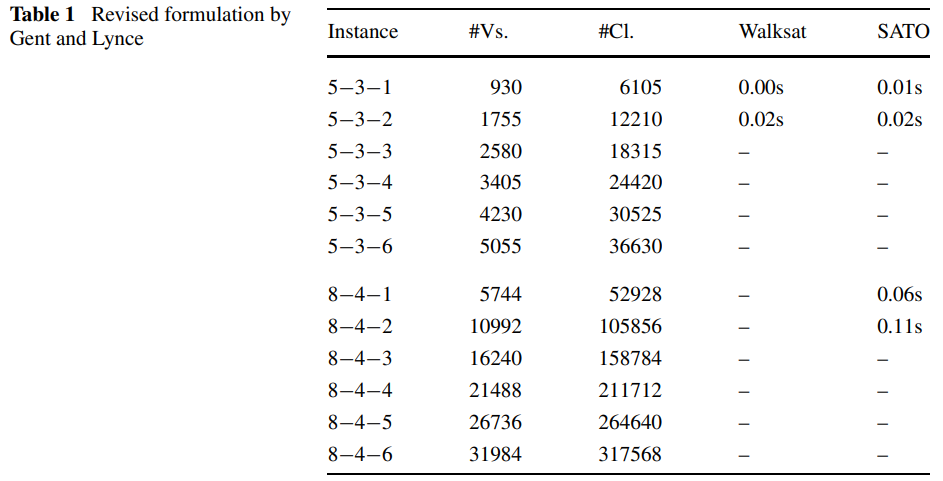
\includegraphics[width=0.8\textwidth]{figures/gent_lynceSAT.png}
    \caption{Rendimiento del modelo SAT original}
    \label{fig:sat_original}
\end{figure}

\begin{figure}[h]
    \centering
    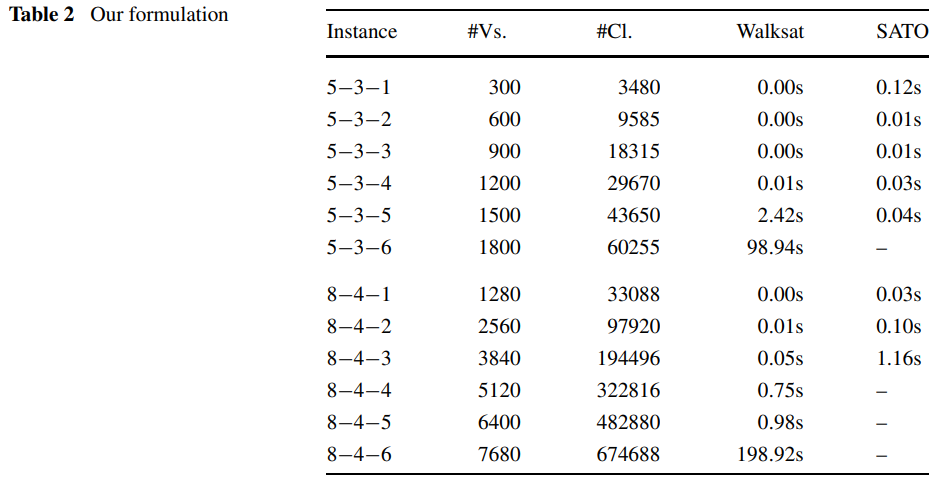
\includegraphics[width=0.8\textwidth]{figures/triksaSAT.png}
    \caption{Rendimiento del modelo SAT modificado}
    \label{fig:sat_triska}
\end{figure}

Como se puede observar, la formulación modificada tiene muchas menos variables para cada instancia, aunque para algunos casos la cantidad de restricciones es mayor. La columna Walksat corresponde al tiempo promedio en segundos hasta que se encuentra una solución factible en 10 intentos. La columna SATO muestra la cantidad de segundos hasta que se encuentra una solución cualquiera, promediada en más de 10 ejecuciones para reducir la varianza de los tiempos de ejecución medidos. El símbolo "-" significa que no se encontraron soluciones en el tiempo límite. El modelo modificado (no así el original) pudo encontrar soluciones a todas las instancias dadas, lo que hace claro que las modificaciones realizadas pueden resultar en una mejora en rendimiento para resolver SGP.

Un modelo parcialmente booleano (PB) propuesto en \cite{lester21pb}, donde se afirma que la restricción de socialización es $\mathcal{O}(g^4p^2w^2)$ lo cual para un número grande de jugadores se encontró que únicamente generar las restricciones es lento. Por esto mismo, se optó por una formulación PB, la cual asume que no necesariamente encuentra una solución óptima, si es que dejó de hacer progreso, al menos encontrará una solución localmente óptima. Recordemos del estado del arte que el propósito de esta investigación era organizar un torneo de Mahjong, donde hay que considerar otro tipo de generalizaciones (en este caso la orientación del viento, turnos en la mesa, rotaciones de dealers, entre otros). Se presenta una codificación monolítica parcialmente booleana, donde se considera que $n=gp$ como el número de jugadores. Las restricciones usan las siguientes variables binarias, donde $h,i,j \in [1,n]$ con $j>i$, $h\neq i$ y $h\neq j$, $k\in [1,g]$, $l\in [1,w]$ y $s \in [1,p]$:

\begin{itemize}
    \item $P_{ikl}$: 1 si $i$ juega en el grupo $k$ en la sesión $l$, 0 e.o.c
    \item $S_{ikls}$: 1 si $i$ juega en el grupo $k$ en la sesión $l$ en la posición de asiento $s$, 0 e.o.c
    \item $M_{ijl}$: 1 si $i$ y $j$ se encuentran en la sesión $l$, 0 e.o.c
    \item $C_{ij}$: 1 si $i$ y $j$ compiten entre ellos en alguna sesión, 0 e.o.c
    \item $D_{ijh}$: 1 si ambos $i$ y $j$ compiten (indirectamente) contra $h$, 0 e.o.c  
\end{itemize}

Luego, para la cardinalidad del espacio de búsqueda se tiene $2^{ngw}\cdot 2^{ngwp}\cdot 2^{\frac{n(n-1)w}{2}} \cdot 2^{\frac{n(n-1)}{2}} \cdot 2^{\frac{n(n-1)(n-2)}{2}} = 2^{ngw(1+p)}\cdot2^{\frac{n(n-1)}{2}(w+n-1)}$. Cada potencia de 2 de la primera parte corresponde al espacio de búsqueda de cada variable según su orden de aparición en el listado anterior. Para $P_{ikl}$ se tendrán $ngw$ variables, mientras que para $S_{ikls}$ serían $ngwp$. Para el resto hay que usar combinatorias, en $M_{ijl}$ sabemos que $j>i$ (aprovechando la simetría esto ayuda a reducir el espacio de búsqueda), por ende tenemos $\binom{n}{2}=\frac{n!}{(n-2)!2!}=\frac{n(n-1)(n-2)!}{(n-2)!2} = \frac{n(n-1)}{2}$ y agregándole la sesión $l$ tenemos un total de $\frac{n(n-1)w}{2}$ variables. Para $C_{ij}$ seguimos el mismo procedimiento anterior (menos las sesiones) y llegaremos a un total de $\frac{n(n-1)}{2}$ variables. En $D_{ijh}$ podemos aprovechar el mismo resultado, como $h\neq i$ y $h\neq j$ se tienen $n-2$ posibilidades, por lo que hay $\frac{n(n-1)(n-2)}{2}$ variables.

Para las direcciones del viento se codifica Este como 1, Sur como 2, etc. Las restricciones planteadas en el paper son las siguientes:\\\\
Cada jugador juega en exactamente un grupo en cada sesión:
\begin{equation}
    \sum_{i} P_{ikl} = p \quad \forall k,l
    \label{eq:9}
\end{equation}
\\
Opcionalmente, para romper simetrías, ordenar a los jugadores secuencialmente en la primera sesión:
\begin{equation}
    P_{i\lceil i/g \rceil 1} = 1 \quad \forall i
    \label{eq:10}
\end{equation}
\\
Si $i$ y $j$ juegan en el mismo grupo en la misma sesión, entonces deben encontrarse en esa sesión:
\begin{equation}
    -P_{ikl} -P_{jkl} + M_{ijl} \geq -1 \quad \forall i,j,k,l
    \label{eq:11}
\end{equation}
\\
Además deben encontrarse a lo más una vez en todas las sesiones:
\begin{equation}
    \sum_l -M_{ijl} \geq -1 \quad \forall i,j
    \label{eq:12}
\end{equation}
\\
$i$ y $j$ compitieron solo si jugaron en el mismo grupo en cualquier sesión:
\begin{equation}
    -C_{ij} + \sum_{k,l} P_{ikl}P_{jkl} \geq 0 \quad \forall i,j
    \label{eq:13}
\end{equation}
\\
$i$ y $j$ compitieron indirectamente vía $h$ solo si ambos compitieron con h:
\begin{equation}
    C_{\min(i,h)\max(i,h)} + C_{\min(j,h)\max(j,h)} - 2D_{ijh} \geq 0 \quad \forall i,j,h
    \label{eq:14}
\end{equation}
\\
$i$ y $j$ deben competir directamente, o competir indirectamente $d$ veces ($d$ configurable):
\begin{equation}
    d\cdot C_{ij} + \sum_h D_{ijh} \geq d \quad \forall i,j
    \label{eq:15}
\end{equation}
\\
Cada jugador debe jugar en cada grupo a lo más una vez en todas las sesiones:
\begin{equation}
    \sum_l -P_{ikl} \geq -1 \quad \forall i,k
    \label{eq:16}
\end{equation}
\\
Si $i$ se sienta en una posición en un grupo, debe jugar en ese grupo:
\begin{equation}
    -S_{ikls} + P_{ikl} \geq 0 \quad \forall i,k,l,s
    \label{eq:17}
\end{equation}
\\
Si $i$ juega en un grupo, debe sentarse en alguna de sus posiciones:
\begin{equation}
    -P_{ikl} +\sum_s S_{ikls} \geq 0 \quad \forall i,k,l
    \label{eq:18}
\end{equation}
\\
Exactamente un jugador debe sentarse en cada puesto:
\begin{equation}
    \sum_i S_{ikls} = 1 \quad \forall k,l,s
    \label{eq:19}
\end{equation}
\\
Cada jugador debe jugar en cada posición (aproximadamente) el mismo número de veces:
\begin{equation}
\begin{aligned}
    \sum_{k,l} S_{ikls} \geq \lfloor w/p \rfloor \quad \forall i,s \\
    \sum_{k,l} -S_{ikls} \geq -\lceil w/p \rceil \quad \forall i,s
    \label{eq:20}
\end{aligned}
\end{equation}

Las restricciones \ref{eq:9} a \ref{eq:13} provienen de otro paper mencionado, donde el objetivo es maximizar la socialización entre jugadores (\cite{csplib:prob010}), mientras que el resto son originales de la investigación de \cite{lester21pb}. Tambien se advierte que, en la práctica, no siempre va a ser posible satisfacer todas las restricciones simultaneamente, ya sea porque no existe solución, o porque el solver no puede encontrar uno. En estos casos, las restricciones \ref{eq:12}, \ref{eq:15}, \ref{eq:16} o \ref{eq:20} se pueden volver blandas.

Para codificar una restricción para el balance del viento se usan variables $W_{ils}$ que son 1 solamente si el jugador $i$ se encuentra en la posición $s$ en la sesion $l$. Esto agranda la cardinalidad del espacio de búsqueda en $2^{nwp}$ veces. Las restricciones son como sigue:\\
Cada jugador debe tener un asiento:
\begin{equation}
    \sum_s W_{ils} = 1 \quad \forall i,l
    \label{eq:21}
\end{equation}
\\
Exactamente un jugador en un grupo puede tomar cada asiento:
\begin{equation}
    \sum_{\{i \hspace{2pt} \vline \hspace{1pt} P_{ikl}\}} W_{ils} = 1 \quad \forall k,l,s
    \label{eq:22}
\end{equation}
\\
Cada jugador debe jugar en cada posición (aproximadamente) la misma cantidad de veces:
\begin{equation}
\begin{aligned}
    \sum_{l} W_{ils} \geq \lfloor w/p \rfloor \quad \forall i,s \\
    \sum_{l} -W_{ils} \geq -\lceil w/p \rceil \quad \forall i,s
    \label{eq:23}
\end{aligned} 
\end{equation}

Los resultados de este modelo se presentaron al final de la sección anterior.

Generalmente el problema siempre viene con una instancia en que la cantidad de semanas en las que dura el torneo son fijas. Aunque hay otros casos en donde se quiere saber hasta cuándo se podría extender el juego tenemos que tener claro que tipo de restricciones entran en juego. Por ejemplo en la instancia original del problema ($8-4-w$) \cite{triska2012effective} menciona que la cantidad de semanas no puede ser más de 10 ya que un jugador se tendría que emparejar con 33 jugadores para hacer esto posible, lo cual sabemos que no lo es pues la instancia solo tiene 32 jugadores.

\section{Representación} \label{rep}

En este caso particular es conveniente usar una matríz tridimensional que guarde la organización de los grupos a través de las semanas, algo similar a lo siguiente:
\begin{figure}[h]
    \centering
    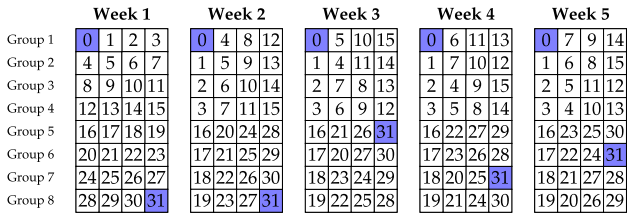
\includegraphics[width=\textwidth]{figures/triskarep.png}
    \caption{Representación de una configuración, sacada de \cite{triska2012effective}}
    \label{fig:representation}
\end{figure}
\\
Dentro de nuestro código, esto se verá como sale en la figura \ref{fig:config_cod}.
\begin{figure}[h]
    \centering
    \begin{subfigure}[b]{0.3\textwidth}
        \centering
    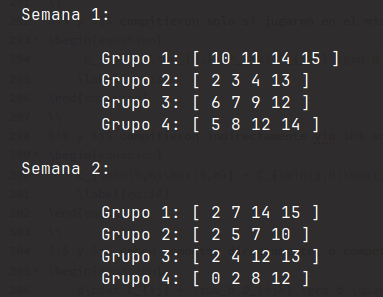
\includegraphics[width=\textwidth]{figures/conf_1.png}

    \end{subfigure}
    \hspace{1mm}
    \begin{subfigure}[b]{0.3\textwidth}
        \centering
        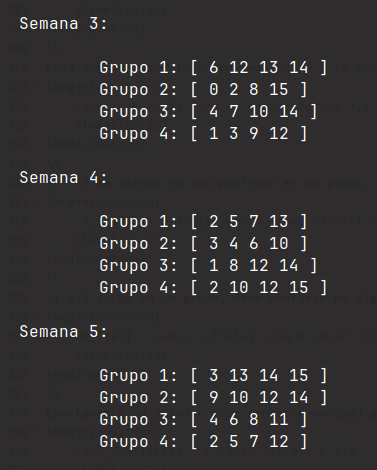
\includegraphics[width=\textwidth]{figures/conf_2.png}
    \end{subfigure}
        \caption{Representación de una configuración en el código propuesto. La instancia mostrada es la 4-4-5.}
    \label{fig:config_cod}
\end{figure}

Se eligió esta representación ya que era lo más fácil para tratar con colisiones de jugadores (como repeticiones de grupos, jugadores que se repiten dentro de la misma semana, entre otros).
Cabe recalcar que también tenemos un listado que enumera los jugadores desde el $0$ hasta el $g\cdot p - 1$ que nos será de útilidad para los algoritmos implementados.

\section{Descripción del algoritmo} \label{algdesc}

\subsection{Construcción}

Usamos una combinación de una heurística greedy basada en el concepto de grado de libertad (visto anteriormente en \cite{triska2012effective}) con otras 2 propuestas que también dan buenos resultados. Se proponen 3 algoritmos greedy para hacer la construcción de una solución inicial; en el primero, iteramos sobre las semanas y grupos dentro de cada semana, para cada grupo queremos insertar el par de jugadores que tengan el mayor grado de libertad posible. Una vez seleccionados estos jugadores se les agrega a una lista de pares restringidos, la cuál nos sirve para no generar la misma tupla de jugadores en semanas distintas, además de ser agregados cada uno por independiente a una lista de jugadores restringidos para los grupos de esa semana en particular, obligando a que un jugador juegue únicamente una vez a la semana. A este algoritmo se le agrega una componente de alietoriedad con una probabilidad $p_{insertion}$; su modo de uso es que elegimos si insertamos en el grupo actual el segundo jugador del par de jugadores elegidos en base a la máxima libertad con probabilidad $p_{insertion}$. Con probabilidad $1-p_{insertion}$ elegimos un jugador al azar del listado de jugadores disponibles. Si la cantidad de jugadores por grupo es impar, se sigue la misma estrategia hasta llegar a la última casilla donde se vuelve a aplicar la probabilidad para elegir el último jugador del grupo. En la figura \ref{fig:grfree} podemos apreciar una configuración inicial construida con esta heurística. Los otros dos algoritmos son más directos: Para el greedy aleatorio simplemente sacamos una muestra aleatoria de tamaño $p$ del arreglo de los jugadores de la instancia en específico; aquí la idea es que se generen las mayores colisiones posibles para que la búsqueda local pueda encontrar buenas soluciones. El otro algoritmo propuesto es un greedy a fuerza bruta; iteramos en cada una de las semanas y en los grupos de la semana en específico. A cada grupo le vamos asignando los jugadores enumerados de mayor a menor, repitiéndose los mismos grupos durante todas las semanas. La gracia de este último es que aunque venga con colisiones entre grupos de distintas semanas, cada jugador juega una sola vez y le da un buen punto de partida a la búsqueda local (como veremos más adelante, se obtienen buenos resultados para este). Las figuras \ref{fig:bruteforce} y \ref{fig:randgr} muestran configuraciones iniciales obtenidas con fuerza bruta y aleatoriamente, respectivamente.  

\begin{figure}[h]
    \centering
    \begin{subfigure}[b]{0.3\textwidth}
        \centering
        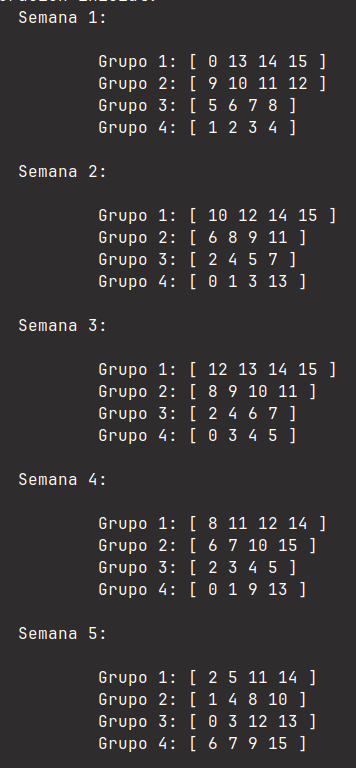
\includegraphics[width=\textwidth]{figures/greedy_freedom.png}
        \caption{Configuración obtenida usando grado de libertad.}
        \label{fig:grfree}
    \end{subfigure}
    \hspace{0.5mm}
    \begin{subfigure}[b]{0.3\textwidth}
        \centering
        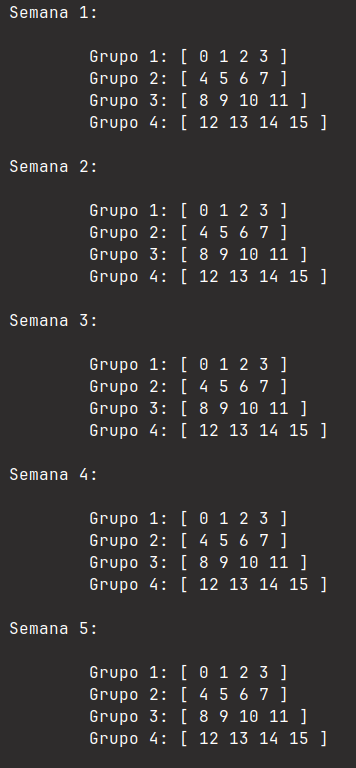
\includegraphics[width=\textwidth]{figures/greedy_brute.png}
        \caption{Configuración obtenida usando fuerza bruta.}
        \label{fig:bruteforce}
    \end{subfigure}
    \hspace{0.5mm}
    \begin{subfigure}[b]{0.3\textwidth}
        \centering
        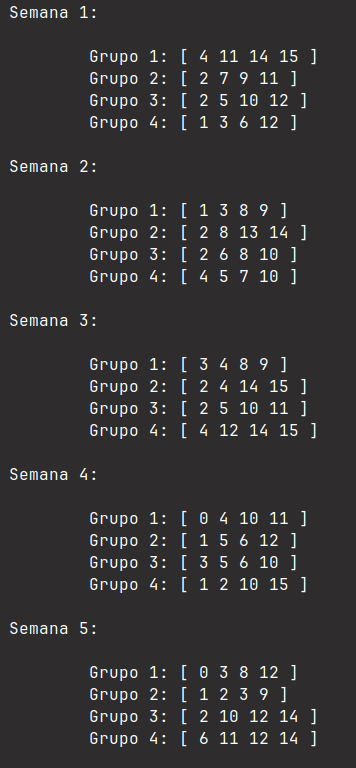
\includegraphics[width=\textwidth]{figures/greedy_random.png}
        \caption{Configuración obtenida usando greedy aleatorio.}
        \label{fig:randgr}
    \end{subfigure}

    \caption{Distintas configuraciones iniciales para la instancia 4-4-5.}
    \label{fig:greedys}
\end{figure}

\subsection{Búsqueda local}

Para búsqueda local implementamos un algoritmo Hill Climbing tanto con mejor mejora como con alguna mejora. La implementación de cada uno es bastante simple en lo que es el algoritmo en sí: Para mejor mejora, generamos el vecindario de la solución actual (en la siguiente sección entraremos en más detalles sobre cómo se construye el vecindario) y después evaluamos cada uno de los vecinos. Si la mejor evaluación encontrada es mejor o igual a la que ya teníamos la nueva solución será la que tuvo mejor evaluación entre todos los vecinos. El proceso se repite hasta que alcancemos el límite de iteraciones. Para alguna mejora la idea es básicamente la misma pero en vez de evaluar todo el vecindario solo llego hasta aquel vecino que tiene mejor evaluación que la solución actual. 
La función de evaluación usada es la siguiente:
\begin{center}
    \# Colisiones dentro de un único grupo $\cdot g \cdot p$ + \# Colisiones de grupos repetidos en semanas distintas $\cdot g$ + \# Colisiones de jugadores dentro de la semana  
\end{center}

El primer tipo de colisión se da cuando un jugador es asignado más de una vez dentro del mismo grupo (físicamente imposible, por lo que la penalización es más dura); el segundo tipo de colisión hace referencia a aquellos grupos de jugadores que se repiten en semanas distintas (muy útil para guiar la búsqueda cuando la solución inicial se generó aleatoriamente). El tercer y último tipo se explica por sí mísmo: hace referencia a la restricción de que un jugador juega a lo más una vez por semana, si este aparece más de una vez dentro de esta se deben ir sumando la cantidad de veces que el jugador aparece en la misma semana. 

Vale la pena mencionar que el algoritmo también tiene soporte para realizar restarts; cuando se hace un restart se utiliza el mismo algoritmo constructor para generar una nueva solución. Cabe recalcar que hacer uso de restart en fuerza bruta no tiene mucho sentido ya que esta no tiene una componente aleatoria que pueda hacer que generemos distintas soluciones iniciales. En la siguiente sección discutiremos de qué nos sirve hacer restart aunque se haya escogido la heurística por fuerza bruta.

\subsection{Generación de vecindario}

Para generar el vecindario de la búsqueda local se tomo en consideración un enfoque más estocástico. Se introduce otro parámetro que nos permite elegir la probabilidad de hacer un swap entre jugadores distintos \textbf{en la misma semana} con una probabilidad $p_{swap}$. Con probabilidad $1-p_{swap}$ hacemos un swap entre jugadores distintos de semanas distintas, lo que nos permite una gama más amplia de vecinos, aunque al ser un proceso basado en probabilidades es más difícil controlar la calidad de las soluciones en las que nos estámos moviendo. Esta es también la razón por la cuál hayan casos en los que conviene hacer restarts aunque la técnica constructora sea a fuerza bruta: igualmente podemos obtener vecinos distintos.

\section{Experimentos} \label{exps}

Los experimentos fueron realizados en un notebook Acer Aspire 5 el cuál tiene un procesador Intel Core i3-10110U de 4.1 GHz y una memoria RAM de 11.775 MiB, el sistema operativo es Ubuntu 22.04 LTS. Se trató de encontrar la mejor configuración de parámetros para cada una de las instancias con un script de python que usa múltiples threads para ejecutar (de fondo) el programa con distintas combinaciones de parámetros para una instancia dada. Se determino un promedio de 20 parámetros generados aleatoriamente por el script mediante prueba y error y limitaciones de la máquina (ver instrucciones de ejecución en README). Esto se hizo de esta forma para poder aprovechar al máximo la capacidad computacional disponible. Al final de la ejecución de una instancia en específico se da a conocer el porcentaje de mejora de la solución después de la búsqueda local, por lo que con este script se busca maximizar este porcentaje al 100\%.  

\section{Resultados} \label{results}

En la siguiente tabla podemos ver, por cada instancia disponible, el mayor porcentaje de mejora alcanzado en conjunto a sus respectivos parámetros; el porcentaje de mejora se calcula en base a $(eval_i - eval_{HC}) / eval_i \cdot 100$, es decir, que tanto disminuyó la evaluación de la configuración después de aplicar Hill Climbing, el valor ideal es de un 100\% ya que se espera que no hayan colisiones en la configuración final. La cantidad de restarts e iteraciones necesarias para hacer un restart se dejaron en 0 ya que usualmente no ayudan mucho a mejorar la solución (en muchos casos la empeoran).

\begin{center}
\begin{table}[!h]
\begin{tabular}{|c|c|c|c|c|c|c|c|c|}
\hline
   Instancia  & \# de iteraciones & Modo de HC & Modo Greedy  & $p_{swap}$ & $p_{insertion}$ & Mejora (\%) \\
   \hline
    $4-2-7$ & 305 & Alguna Mejora & Bruto & 0.1552 & 0.2275 & 88.5417 \\
    \hline
    $4-4-5$ & 468 & Alguna Mejora & Bruto & 0.3 & 0.8 & 100\\
    \hline
    $5-2-9$ & 136 & Alguna Mejora & Bruto & 0.2908 & 0.6710 & 91\\
    \hline
    $5-3-7$ & 486 & Alguna Mejora & Bruto & 0.3 & 0.8 & 100 \\
    \hline
    $6-3-8$ & 480 & Mejor Mejora & Bruto & 0.3 & 0.8 & 100 \\
    \hline
    $7-3-10$ & 343 & Mejor Mejora & Bruto & 0.3 & 0.8 & 100 \\
    \hline
    $7-4-9$ & 219 & Alguna Mejora & Bruto & 0.3 & 0.8 & 100 \\
    \hline
    $8-4-10$ & 260 & Alguna Mejora & Bruto & 0.3 & 0.8 & 100 \\
    \hline
\end{tabular}
\caption{Parámetros ideales para cada instancia promediados con 10 ejecuciones.}
\end{table}
\end{center}

Como podemos observar todos encontraban mejores soluciones al usar un greedy a fuerza bruta antes que con los otros. En otras repeticiones del mismo experimento también aparecía el greedy con grados de libertad; esta variabilidad entre los greedy más convenientes se debe a la aleatoriedad con la que se generan estos parámetros, por lo que se recomienda jugar con la cantidad de parámetros que se generan (esto obviamente tiene un costo en computación). Para los parámetros que se muestran en la tabla, los tiempos de ejecución promedio se pueden ver en el cuadro \ref{table:2}.

\begin{center}
\begin{table}[!h]
\centering
    \begin{tabular}{c|c}
        Instancia & Tiempo de ejecución de HC (s) \\
    \hline
         $4-2-7$ & 1.792 \\
         $4-4-5$ & 4.036\\
         $5-2-9$ & 1.677 \\
         $5-3-7$ & 8.072\\
         $6-3-8$ & 16.134 \\
         $7-3-10$ & 25.948 \\
         $7-4-9$ & 12.004 \\
         $8-4-10$ & 23.528
    \end{tabular}
    \caption{Tiempos de ejecución de HC para cada instancia, promediado en 5 ejecuciones.}
    \label{table:2}
\end{table}
\end{center}

\section{Conclusiones} \label{conc}

Podemos concluir que SGP es un problema que ha sido muy explorado en el campo de la optimización combinatoria no solo para resolver el problema en sí sino que también para instancias o generalizaciones que pueden ser reducibles a SGP y ser resueltas con algunos de los métodos mencionados a lo largo de esta investigación. La técnica que usemos depende netamente de la formulación que se le da al problema, como vimos anteriormente a veces un modelo más complejo puede obtener mejores soluciones bajo el contexto en el que se estudia en comparación con alguna extrapolación a otros casos, donde la misma complejidad del modelo resulta ineficiente y se debe optar por opciones más simples pero con heurísticas más creativas para resolver el problema. El enfoque general que se le da a un problema de este tipo es tratar de aprovechar al máximo sus simetrías para poder hacer un modelo y técnica de resolución que use bien toda la información aportada y mejorar su rendimiento al máximo posible, lo que lo convierte en un estándar para comparar técnicas de resolución. Es claro que un enfoque de búsqueda local con una inicialización greedy es la que da mejores resultados a la hora de comparar con los otros algoritmos explorados, que a pesar de tener un peor rendimiento siguen siendo bastante buenos ya que nos dan otro punto de vista que nos puede ser útil a la hora de querer implentar soluciones innovadoras. 

Se propuso una metodología para poder resolver el problema desde un enfoque un tanto más automatizado el cuál es bastante útil para poder encontrar los parámetros ideales para correr nuestro programa. La heurística por fuerza bruta es la que más predomina para poder encontrar soluciones de calidad aunque el factor de la cantidad de iteraciones y el modo en que se realiza Hill Climbing también toman peso en el porcentaje de mejora de una solución. Todos estos resultados son coherentes con respecto a las conclusiones que pudimos obtener en el estado del arte del problema.

\printbibliography

\end{document} 